\documentclass[a4,10pt]{aleph-notas}

% -- Paquetes adicionales
\usepackage{enumitem}
\usepackage{aleph-comandos}
\usepackage{quantikz}

% -- Datos
\institucion{Proyecto Alephsub0}
\asignatura{Computación Cuántica}
\tema{Teleportación cuántica}
\autor{Andrés Merino}
\fecha{Julio 2026}

\fuente{montserrat}
\logouno[4.5cm]{Logos/LogoAlephsub0-02}
\definecolor{colordef}{cmyk}{0.81,0.62,0.00,0.22}

% -- Comandos adicionales
\newtheorem*{prob}{Problema}
    \tcolorboxenvironment{prob}{%
        color=colordef,recuadrost,colback=colordef!7,drop fuzzy shadow
    }

\begin{document}


\encabezado

La teleportación cuántica es un protocolo que permite transferir un estado
cuántico desconocido desde un cúbit de Alice hacia un cúbit de Bob,
utilizando un par entrelazado compartido y el envío de dos bits de
información clásica.

La idea es:
\begin{itemize}
    \item Alice posee un cúbit en el estado desconocido
    \[
        \ket{\psi}=\alpha\ket{0}+\beta\ket{1},
        \qquad
        |\alpha|^2+|\beta|^2=1.
    \]
    \item Alice y Bob comparten previamente un par entrelazado. Alice conserva
    uno de los cúbits del par y Bob conserva el otro.
    \item Alice aplica operaciones sobre su cúbit original y sobre su parte del
    par entrelazado, y luego mide ambos cúbits.
    \item Alice envía a Bob los dos bits clásicos obtenidos en la medición.
    \item Bob aplica correcciones condicionadas por esos bits y recupera el
    estado original \(\ket{\psi}\).
\end{itemize}

El circuito de teleportación cuántica es:
\begin{center}
    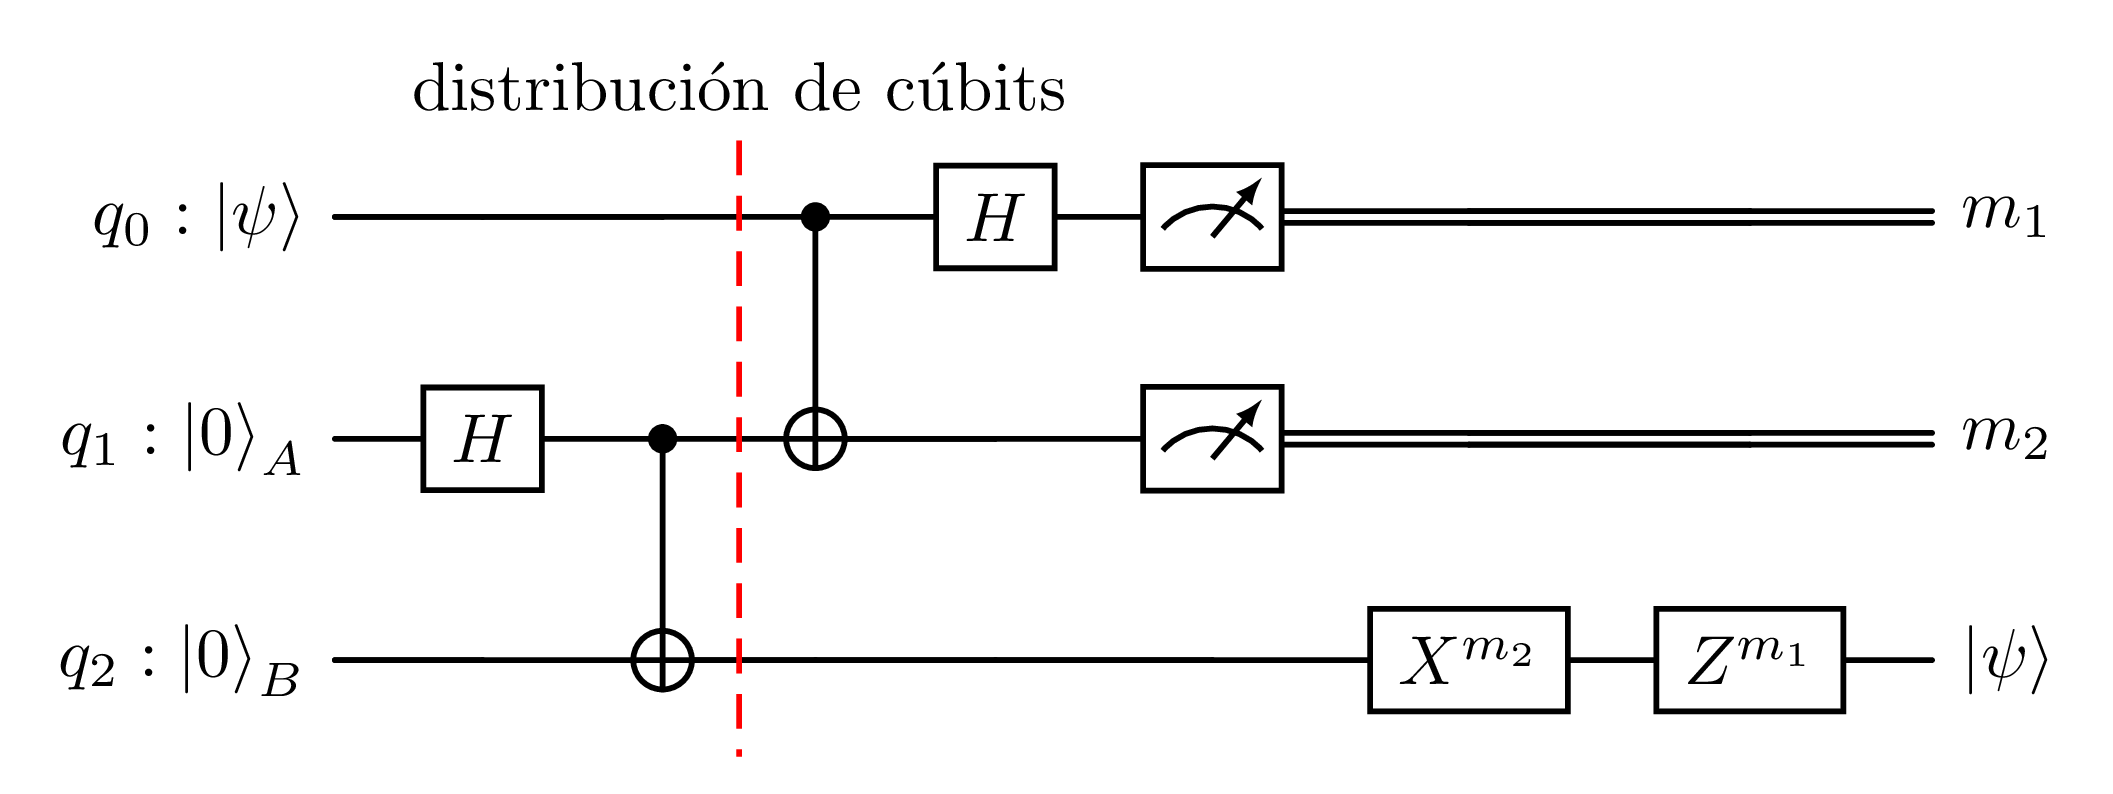
\includegraphics[width=0.75\textwidth]{imagen.png}
\end{center}

\begin{prob}
    Realizar la derivación matemática de la teleportación cuántica.
\end{prob}

\begin{proof}
    Sean \(q_0\), \(q_1\) y \(q_2\) los cúbits del circuito. El cúbit \(q_0\) contiene el estado desconocido que se desea teleportar:
    \[
        \ket{\psi}=\alpha\ket{0}+\beta\ket{1},
    \]
    donde
    \[
        |\alpha|^2+|\beta|^2=1.
    \]
    Los cúbits \(q_1\) y \(q_2\) se encuentran inicialmente en el estado \(\ket{0}\). Por tanto, el estado inicial del sistema es
    \[
        \ket{\Psi_0}=\ket{\psi}\ket{00}=\left(\alpha\ket{0}+\beta\ket{1}\right)\ket{00}.
    \]
    Alice posee los cúbits \(q_0\) y \(q_1\), mientras que Bob posee el cúbit \(q_2\).

    Consideremos los siguientes pasos del circuito:
    \begin{center}
        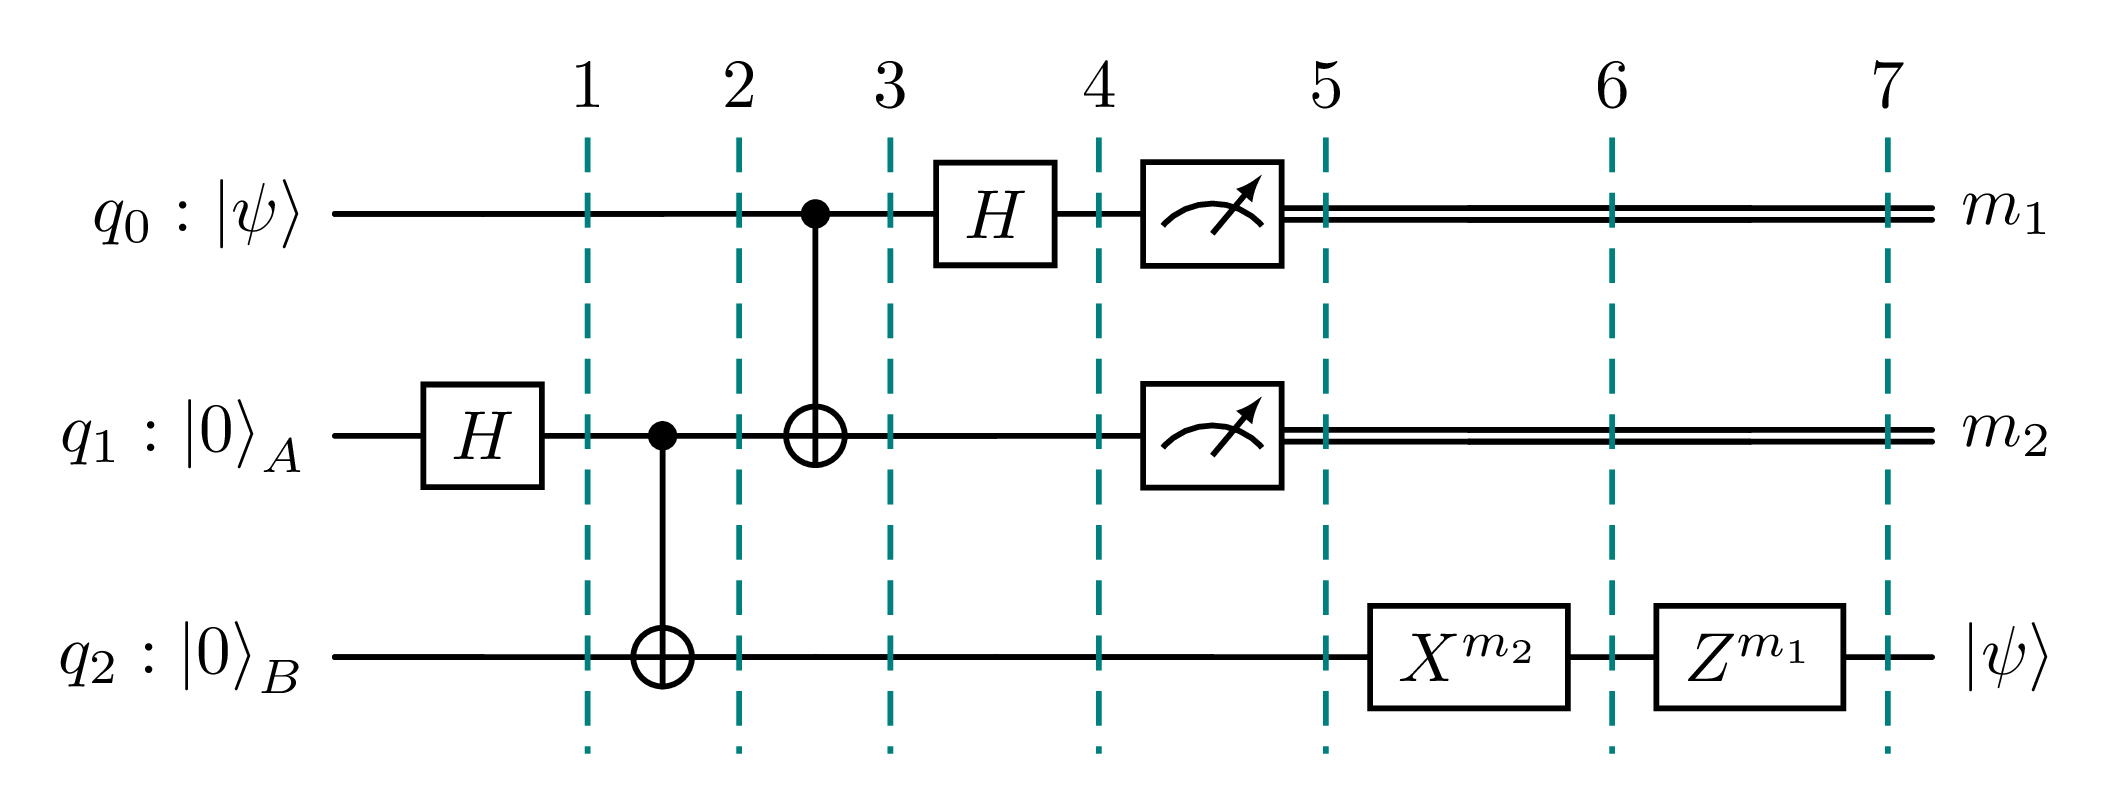
\includegraphics[width=0.8\textwidth]{imagen2.png}
    \end{center}

    \begin{itemize}
        \item \textbf{Paso 1.} Se aplica la compuerta Hadamard al cúbit \(q_1\):
        \[
            \ket{\Psi_1}=(I\otimes H\otimes I)\ket{\Psi_0}.
        \]
        Como
        $
            H\ket{0}=\frac{1}{\sqrt{2}}\left(\ket{0}+\ket{1}\right),
        $
        se obtiene
        \begin{align*}
            \ket{\Psi_1}
            &=\left(\alpha\ket{0}+\beta\ket{1}\right)\otimes\frac{1}{\sqrt{2}}\left(\ket{0}+\ket{1}\right)\otimes\ket{0}\\
            &=\frac{1}{\sqrt{2}}\left(\alpha\ket{000}+\alpha\ket{010}+\beta\ket{100}+\beta\ket{110}\right).
        \end{align*}

        \item \textbf{Paso 2.} Se aplica una compuerta CNOT, utilizando \(q_1\) como control y \(q_2\) como objetivo:
        \[
            \ket{\Psi_2}=\operatorname{CNOT}_{1,2}\ket{\Psi_1}.
        \]
        Por tanto,
        \[
            \ket{\Psi_2}=\frac{1}{\sqrt{2}}\left(\alpha\ket{000}+\alpha\ket{011}+\beta\ket{100}+\beta\ket{111}\right).
        \]
        El segundo cúbit se entrega a Alice y el tercero a Bob.

        \item \textbf{Paso 3.} Alice aplica una compuerta CNOT, utilizando \(q_0\) como control y \(q_1\) como objetivo:
        \[
            \ket{\Psi_3}=\operatorname{CNOT}_{0,1}\ket{\Psi_2}.
        \]
        En consecuencia,
        \[
            \ket{\Psi_3}=\frac{1}{\sqrt{2}}\left(\alpha\ket{000}+\alpha\ket{011}+\beta\ket{110}+\beta\ket{101}\right).
        \]

        \item \textbf{Paso 4.} Alice aplica la compuerta Hadamard al cúbit \(q_0\):
        \[
            \ket{\Psi_4}=(H\otimes I\otimes I)\ket{\Psi_3}.
        \]
        Usando que
        $
            H\ket{0}=\frac{\ket{0}+\ket{1}}{\sqrt{2}},
            $ $H\ket{1}=\frac{\ket{0}-\ket{1}}{\sqrt{2}},
        $
        se obtiene
        \begin{align*}
            \ket{\Psi_4}=\frac{1}{2}\big(&\alpha\ket{000}+\alpha\ket{100}+\alpha\ket{011}+\alpha\ket{111}\\
            &+\beta\ket{010}-\beta\ket{110}+\beta\ket{001}-\beta\ket{101}\big).
        \end{align*}
        Agrupando los términos de acuerdo con los dos primeros cúbits,
        \begin{align*}
            \ket{\Psi_4}=\frac{1}{2}\big(&\ket{00}\left(\alpha\ket{0}+\beta\ket{1}\right)+\ket{01}\left(\alpha\ket{1}+\beta\ket{0}\right)\\
            &+\ket{10}\left(\alpha\ket{0}-\beta\ket{1}\right)+\ket{11}\left(\alpha\ket{1}-\beta\ket{0}\right)\big).
        \end{align*}
        Utilizando las compuertas de Pauli, esta expresión puede escribirse como
        \[
            \ket{\Psi_4}=\frac{1}{2}\big(\ket{00}\ket{\psi}+\ket{01}X\ket{\psi}+\ket{10}Z\ket{\psi}+\ket{11}XZ\ket{\psi}\big).
        \]

        \item \textbf{Paso 5.} Alice mide los cúbits \(q_0\) u $q_1$ en la base computacional y obtiene los bits clásicos \(m_1,m_2\in\{0,1\}\).

        Después de las mediciones, el cúbit \(q_2\) de Bob se encuentra en uno de los siguientes estados:
        \[
            \begin{array}{c|c}
                m_1m_2 & \text{Estado del cúbit }q_2\\
                \hline
                00 & \ket{\psi}\\
                01 & X\ket{\psi}\\
                10 & Z\ket{\psi}\\
                11 & XZ\ket{\psi}
            \end{array}
        \]
        Es decir,
        \[
            \ket{q_2}=X^{m_2}Z^{m_1}\ket{\psi}.
        \]

        Alice envía a Bob los bits clásicos \(m_1\) y \(m_2\). Estos bits indican las correcciones que Bob debe aplicar.

        \item \textbf{Paso 6.} Bob aplica la compuerta \(X^{m_2}\) al cúbit \(q_2\). Como \(X^2=I\), se obtiene
        \[
            X^{m_2}\ket{q_2}=X^{m_2}X^{m_2}Z^{m_1}\ket{\psi}=Z^{m_1}\ket{\psi}.
        \]
        En particular,
        \[
            \begin{array}{c|c}
                m_1m_2 & \text{Estado después de aplicar }X^{m_2}\\
                \hline
                00 & \ket{\psi}\\
                01 & \ket{\psi}\\
                10 & Z\ket{\psi}\\
                11 & Z\ket{\psi}
            \end{array}
        \]

        \item \textbf{Paso 7.} Finalmente, Bob aplica la compuerta \(Z^{m_1}\). Como \(Z^2=I\), resulta
        \begin{align*}
            Z^{m_1}X^{m_2}\ket{q_2}
            &=Z^{m_1}Z^{m_1}\ket{\psi}\\
            &=\ket{\psi}\\
            &=\alpha\ket{0}+\beta\ket{1}.
        \end{align*}
    \end{itemize}

    En consecuencia, el estado desconocido que se encontraba inicialmente en el cúbit \(q_0\) de Alice queda reconstruido en el cúbit \(q_2\) de Bob. El estado cuántico no se copia: el estado original desaparece como consecuencia de la medición y se reconstruye en el cúbit de Bob mediante el uso de un par entrelazado y la transmisión de dos bits clásicos.
\end{proof}




\end{document}
